\chapter{INTRODUCTION}
\label{chap:intro}

%intro here in one paragraph

The approach of enormous informational collections has put weight on the Mathematics and Statistics people group to reexamine how to apply conventional of investigation and inferencing. Both atmosphere and oceanographic science disciplines are feeling this information blast and are attempting to scale. Extraordinary measures of information are made accessible by administrative offices like \gls{noaa} and \gls{nasa}, and vigorously utilized by mainstream researchers to draw inductions. The customary perception and conveyance instruments can be enhanced to deal with a flood of new information conveyance. The methods used to envision and recover these information should be rethought. Worldwide expectations require current mobile application innovations for expert and novice to imagine and get information rapidly, precisely, and as effortlessly on their hands as could be expected under the circumstances.

Conventional strategies for parsing through a remote/nearby document of records, choosing significant documents, opening the documents and performing examination on a solitary \gls{pc} don't scale with enormous information. Researchers are investing more energy exploring through information as opposed to discovering disclosures. More awful still, beginners as youngsters, specialists, understudies and potential researchers get baffled and abandon utilizing these rich informational indexes. Toolboxes web applications and of course mobile applications are recommended in this proposal to alleviate this weight. Present day \gls{restfull} application configuration gives the network a mobile stick to enable them to swim through the huge information soil.


\section{Background and significance of visualizing spatial data using smart phones}

Government organizations deliver basic information about the country's populace, economy, administrations, agriculture and assets. These organizations are going under expanding weight, both societal and money related in nature, to create and actualize \gls{ict}, inside and encompassing their organizations, supporting another worldview of society and modernization, focused on electronic open administration. In these last years, a surprising accomplishment in the utilization of hand-held portable PCs — cell phones, tablet PCs, Personal Digital Assistants, and scratch pad — has been seen for information gathering in various fields.
Information accumulation is perceived as a standout amongst the most tedious, costly and mistake given errands in any information stock venture. Hand-held PCs hold the potential to lessen the calculated weight, cost, and blunder rate of paper-based strategies for information accumulation anyway there is an absence of proper, redid and specialized minimal effort arrangements. The eminent proceeding with development of the \gls{is} industry makes openings and difficulties for intriguing programming applications advancements and usage. In this sense, Geographic Information Systems \gls{gis} and the electronic open organization administrations come into a typical circle. \gls{gis} information frameworks effectively store and control, join, and interrelate spatial genuine articles (e.g. political limits, streets, offices areas). Spatial information verbalized with other information sources gives proficient intends to arranging, basic leadership, and administration numerous parts of financial exercises which take advantage of a spatial measurement. Portability is a progressive wonder and establishes the most imperative current pattern in \gls{it}, uniquely, the classification of ease arrangements.

Portable figuring frameworks and equipment are changing the manner in which versatile mapping innovation is being utilized by moving \gls{gis} from the work area into the client's hands, giving adaptability in information securing, information precision and uprightness — approval progressively lessening blunders and process costs — more data with significantly less time and exertion, quicker correspondence conventions, and high profitability, making the portability a tempting part of \gls{gis}.

%
\begin{figure}[ht]
  \centering
  \begin{minipage}{4.5in}
    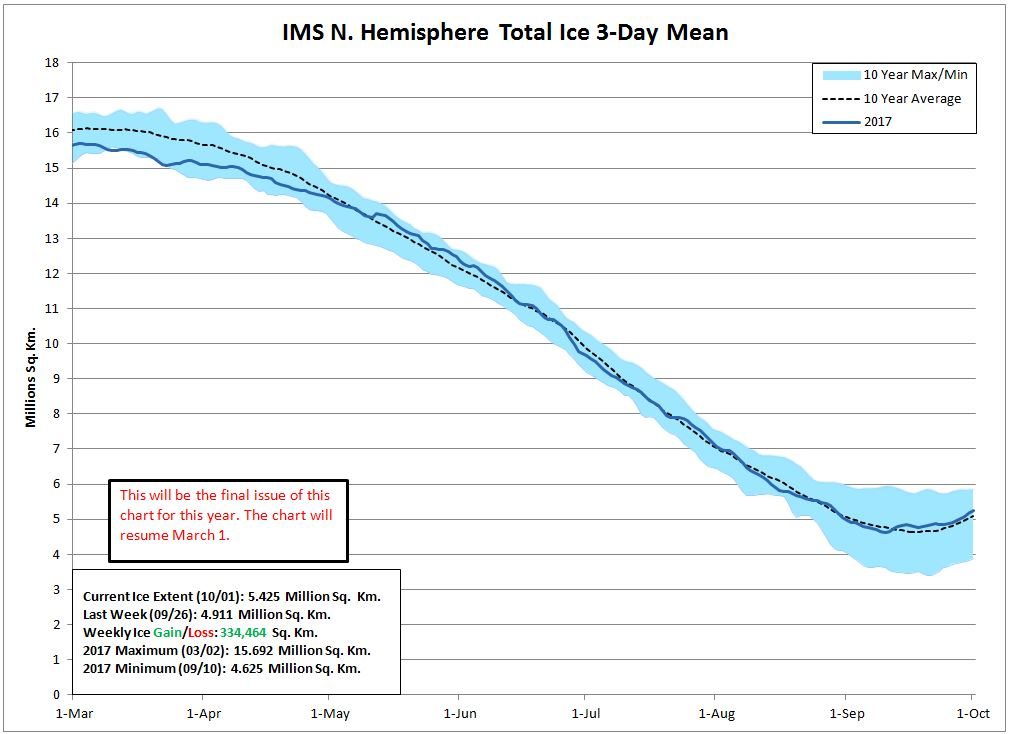
\includegraphics[width=\linewidth]{ims_data.jpg}
    \caption{ \label{fig:nat_ice} Sea and Lake Ice coverage of IMS data using 4 KM resolution. Ice coverages are calculated using a three day running mean from March until September each year. Blue border displays maximum and minimum values for the season. Areas are calculated using the Lambert Azimuthal Equal Area Projection with a WGS84 Datum. \cite{nat_ice}}
  \end{minipage}
\end{figure}
%


\subsection{Past work}
Talking about mobile technologies, Applications began as a stripped down, single-work program to keep running on the telephone and some have kept on being only that. Be that as it may, with advances in equipment and programming the pattern has moved back to having applications accomplish more. This has enabled individuals to supplant a few bits of tech with a solitary cell phone or tablet and, simultaneously, made the information from that gadget a lot more entire. What's more, that information, as opposed to the applications themselves, is the place the genuine world-changing force lies.

Portable application configuration is a solid help for understudy focused registering. By including visual and spatial information in a portable application, understudies can build up a 3-D execution which can furnish the versatile application clients with a virtual ordeal. The improvement of a versatile application for a chronicled cemetery gives a case of how to coordinate database data with visual and spatial information to accomplish s virtual experience. The contextual analysis introduced here, utilizing both Android and \gls{iOS} gadgets, incorporates three sections. At first, a current database was changed over for versatile application get to. This was trailed by plan coordination in help of the coveted versatile application highlights. At last, the incorporation of a picture display, with visual and spatial components, coordinated with the portable application, brought about a convincing versatile application, giving a virtual copy of a genuine visit to the recorded site.

%
\begin{figure}[ht]
  \centering
  \begin{minipage}{4.5in}
    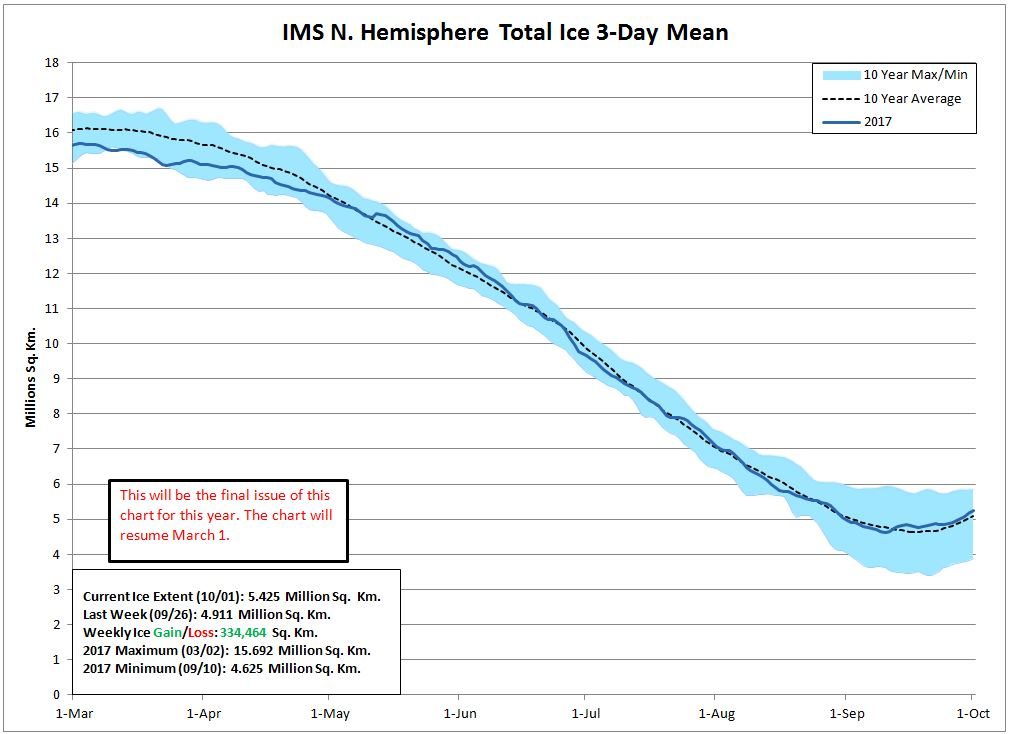
\includegraphics[width=\linewidth]{ims_data.jpg}
    \caption{ \label{fig:nat_ice} Sea and Lake Ice coverage of IMS data using 4 KM resolution. Ice coverages are calculated using a three day running mean from March until September each year. Blue border displays maximum and minimum values for the season. Areas are calculated using the Lambert Azimuthal Equal Area Projection with a WGS84 Datum. \cite{nat_ice}}
  \end{minipage}
\end{figure}
%


\subsection{Current scenario}

Notwithstanding late advances in pen-as well as contact empowered portable gadgets and the quick appropriation of these gadgets in ordinary life, we are a long way from utilizing the maximum capacity of cell phones in fulfilling the developing interest for visual access to information. Despite the fact that the plan space for versatile  information perception is developing out of ordinary practice [14], concentrated research endeavors have not yet risen.





\subsection{Future work for quick visualization and analysis of big data}



\section{Motivation of the VACYD research: crop yield data visualization}



\section{A short summary of the app development method and results}



\begin{figure}[ht]
  \centering
  \begin{minipage}{4.5in}
    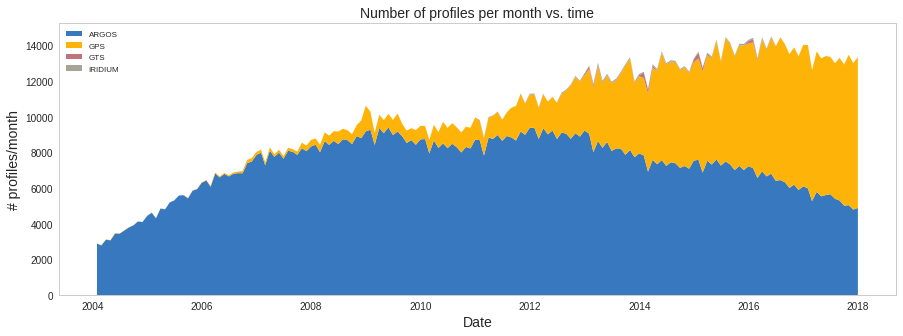
\includegraphics[width=\linewidth]{commTS.png}
    \caption{ \label{fig:commTS} Satalite Communication Type by month. Iridium floats also use the GPS system.}
  \end{minipage}
\end{figure}

\begin{figure}[ht]
  \centering
  \begin{minipage}{4.5in}
    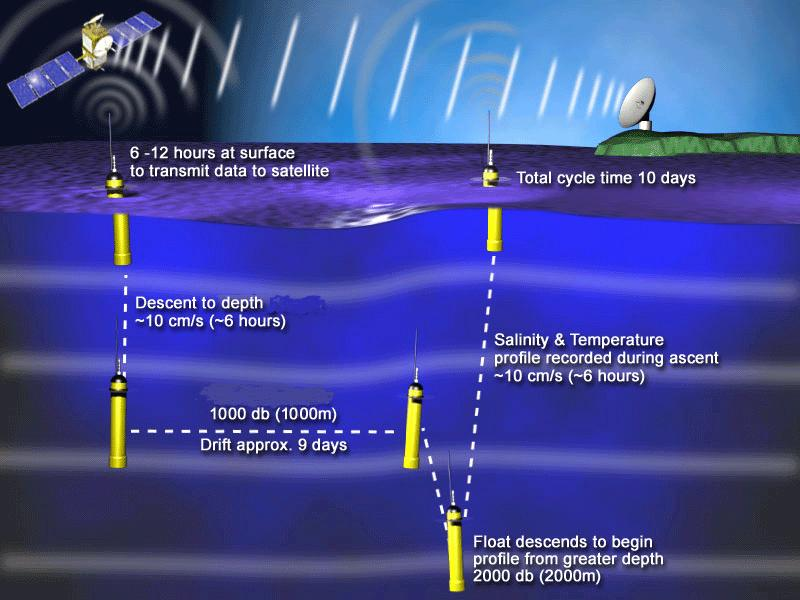
\includegraphics[width=\linewidth]{operation_park_profile.jpg}
    \caption{ \label{fig:argo_cycle} Detail of one profile cycle\cite{argo}}
  \end{minipage}
\end{figure}

\section{Literature review}